\documentclass[a4paper,10pt]{article}
\usepackage[utf8]{inputenc}
\usepackage[T1]{fontenc}
\usepackage[margin=0.75in]{geometry}
\usepackage{paralist}
\usepackage{fancyhdr}
\usepackage{listings}
\usepackage[colorlinks]{hyperref}
\usepackage{amssymb}
\usepackage{amsmath}
% Alwayws load this last
\usepackage{xcolor}
\usepackage{soul}

\def\chpcolor{blue!60}
\def\chpcolortxt{blue!60}
\def\sectionfont{\sffamily\Large}

\setcounter{secnumdepth}{2}

\makeatletter
%Section:
\def\@sectionstrut{\vrule\@width\z@\@height12.5\p@}
\def\@makesectionhead#1{%
  {\par\vspace{20pt}%
   \parindent 0pt\raggedleft\sectionfont
   \colorbox{\chpcolor}{%
     \parbox[t]{25pt}{\color{white}\@sectionstrut\@depth4.5\p@\hfill
       \ifnum\c@secnumdepth>\z@\thesection\fi}%
   }%
   \begin{minipage}[t]{\dimexpr\textwidth-25pt-2\fboxsep\relax}
   \color{\chpcolortxt}\@sectionstrut\hspace{5pt}#1
   \end{minipage}\par
   \vspace{10pt}%
  }
}
\def\section{\@afterindentfalse\secdef\@section\@ssection}
\def\@section[#1]#2{%
  \ifnum\c@secnumdepth>\m@ne
    \refstepcounter{section}%
    \addcontentsline{toc}{section}{\protect\numberline{\thesection}\textbf{#1}}%
  \else
    \phantomsection
    \addcontentsline{toc}{section}{#1}%
  \fi
  \sectionmark{\textbf{#1}}%
  \if@twocolumn
    \@topnewpage[\@makesectionhead{#2}]%
  \else
    \@makesectionhead{\textbf{#2}}\@afterheading
  \fi
}
\def\@ssection#1{%
  \if@twocolumn
    \@topnewpage[\@makesectionhead{#1}]%
  \else
    \@makesectionhead{#1}\@afterheading
  \fi
}
\makeatother




\makeatletter
\def\@makesubsectionhead#1{%
  {\par\vspace{20pt}%
   \parindent 0pt\raggedleft\sffamily\large
   \ifnum\c@secnumdepth>\z@\color{\chpcolortxt}{\thesubsection}\fi%
   %
   \begin{minipage}[t]{\dimexpr\textwidth-2\fboxsep\relax}
   \vspace{-10pt}\color{black}\hspace{5pt}#1
   \end{minipage}\\[-10pt]
   \noindent\rule{\textwidth}{1pt}\par
   \vspace{10pt}%
  }
}
\def\subsection{\@afterindentfalse\secdef\@subsection\@ssection}
\def\@subsection[#1]#2{%
  \ifnum\c@secnumdepth>\m@ne
    \refstepcounter{subsection}%
    \addcontentsline{toc}{subsection}{\protect\numberline{\thesubsection}\textbf{#1}}%
  \else
    \phantomsection
    \addcontentsline{toc}{subsection}{\textbf{#1}}%
  \fi
  \sectionmark{\textbf{#1}}%
  \if@twocolumn
    \@topnewpage[\@makesubsectionhead{\textbf{#2}}]%
  \else
    \@makesubsectionhead{\textbf{#2}}\@afterheading
  \fi
}
\def\@ssection#1{%
  \if@twocolumn
    \@topnewpage[\@makesubsectionhead{\textbf{#1}}]%
  \else
    \@makesubsectionhead{\textbf{#1}}\@afterheading
  \fi
}
\makeatother



\definecolor{codegreen}{rgb}{0,0.6,0}
\definecolor{codegray}{rgb}{0.5,0.5,0.5}
\definecolor{codepurple}{rgb}{0.58,0,0.82}
\definecolor{backcolour}{rgb}{0.95,0.95,0.92}

%Code listing style named "mystyle"
\lstdefinestyle{mystyle}{
  backgroundcolor=\color{backcolour},   commentstyle=\color{codegreen},
  keywordstyle=\color{magenta},
  numberstyle=\tiny\color{codegray},
  stringstyle=\color{codepurple},
  basicstyle=\ttfamily\footnotesize,
  breakatwhitespace=false,         
  breaklines=true,                 
  captionpos=b,                    
  keepspaces=true,                 
  numbers=left,                    
  numbersep=5pt,                  
  showspaces=false,                
  showstringspaces=false,
  showtabs=true,                  
  tabsize=2
}

%"mystyle" code listing set
\lstset{style=mystyle}


\newcommand{\xhdr}[1]{\vspace{5pt}\noindent{\color{blue!60}\textbf{#1}}}


\newcommand{\task}[1]{\xhdr{ {\large $\mathbf{\blacktriangleright}$} \texttt{TASK #1}}}


\usepackage{tcolorbox}
\newtcolorbox{taskbox}{
    arc=0pt,
    boxrule=1pt,
    colback=gray!10,
    colframe=blue!60,
    width=\textwidth,
    halign=left,
}
\usepackage{tikz}
\usetikzlibrary{automata, positioning, arrows}
\usepackage{multicol}





\begin{document}
\tikzset{
->, % makes the edges directed
>=stealth, % makes the arrow heads bold
node distance=2cm, % specifies the minimum distance between two nodes. Change if necessary.
every state/.style={thick, fill=gray!10}, % sets the properties for each ’state’ node
initial text=$ $, % sets the text that appears on the start arrow
}

\sffamily

\begin{center}
\noindent\rule{\textwidth}{1pt}\\[10pt]
{\color{blue!60}{AI539 Natural Language Processing with Deep Learning -- Homework 4}}\\[10pt]
{\LARGE Attention Mechanisms in Sequence-to-Sequence Models}\\[10pt]
\noindent\rule{\textwidth}{1pt}
\end{center}

\noindent\textbf{Overview and Objectives.} In this homework, we'll build some intuitions for scaled dot-product attention and implement a simple attention mechanism for an RNN-based sequence-to-sequence model in a small-scale machine translation task. If you finish early, \emph{work on your projects!}\\

\noindent\textbf{How to Do This Assignment.} The assignment has a few math questions and then walks you through completing the provided skeleton code and analyzing some of the results. Anything requiring you to do something is marked as a "Task" and has associated points listed with it. You are expected to turn in both your code and a write-up answering any task that requested written responses. Submit a zip file containing your completed skeleton code and a PDF of your write-up to Canvas.\\ 

\noindent\textbf{Advice.} Start early. Students will need to become familiar with \texttt{pytorch} for this and future assignments. Extra time may be needed to get used to working remotely on the GPU cluster here. You can also use GPU-enabled runtimes in Colab \url{colab.research.google.com}.

\section{Scaled Dot-Product Attention [8 pts]}
To warm up and start getting more familiar with scaled dot-product attention mechanisms, we'll do some exploratory math first.\footnote{These questions are adapted from CS224n at Stanford because I just liked the originals too much not to use them.} Recall from the lecture the definition of a single-query scaled dot-product attention mechanism. Given a query $\mathbf{q} \in \mathbb{R}^{1\times d}$, a set of candidates represented by keys $\mathbf{k}_1, ... , \mathbf{k}_m \in \mathbb{R}^{1\times d}$ and values $\mathbf{v}_1, ... , \mathbf{v}_m \in \mathbb{R}^{1\times d_v}$, we compute the scaled dot-product attention as:
%
\begin{eqnarray}
\alpha_i &=& \frac{\mbox{exp}\left(~\mathbf{q}\mathbf{k}_i^T / \sqrt d\right)}{\sum_{j=1}^m \mbox{exp}\left(\mathbf{q}\mathbf{k}_j^T / \sqrt d\right)}\\
\mathbf{a} &=& \sum_{j=1}^m \alpha_j \mathbf{v}_j
\end{eqnarray}
%
where the $\alpha_i$ are referred to as attention values (or collectively as an attention distribution). The goal of this section is to get a feeling for what is easy for attention to compute and why we might want something like multi-headed attention to make some computations easier.
%
\vspace{5pt}
\begin{taskbox}
\task{1.1 Copying [2pts]}{ Describe (in one or two sentences) what properties of the keys and queries would result in the output $\mathbf{a}$ being equal to one of the input values $\mathbf{v}_j$. Specifically, what must be true about the query $\mathbf{q}$ and the keys $\mathbf{k}_1, ..., \mathbf{k}_m$ such that $\mathbf{a} \approx \mathbf{v}_j$? (We assume all values are unique -- $\mathbf{v}_i \neq \mathbf{v}_j,~\forall ij$.)}
\end{taskbox}
\vspace{5pt}
%
\vspace{5pt}
\begin{taskbox}
\task{1.2 Average of Two [2pts]}{ Consider a set of key vectors $\{\mathbf{k}_1, ... , \mathbf{k}_m\}$ where all keys are orthogonal unit vectors -- that is to say $\mathbf{k}_i\mathbf{k}_j^T =0,~\forall ij$ and $||\mathbf{k}_i||=1,~\forall i$. Let $\mathbf{v}_a, \mathbf{v}_b \in \{\mathbf{v}_1, ..., \mathbf{v}_m\}$ be two value vectors. Give an expression for a query vector $\mathbf{q}$ such that the output $\mathbf{a}$ is approximately equal to the average of $\mathbf{v}_a$ and $\mathbf{v}_b$, that is to say $\mathbf{a} \approx \frac{1}{2}(\mathbf{v}_a + \mathbf{v}_b)$. You can reference the key vectors corresponding to $\mathbf{v}_a$ and $\mathbf{v}_b$ as $\mathbf{k}_a$ and $\mathbf{k_b}$ respectively. Note that due to the softmax in Eq. 1, it won't ever actually reach this value, but you can make it arbitrarily close by adding a scaling constant to your solution. }
\end{taskbox}
\vspace{5pt}
%
In the previous task, we saw it was
\emph{possible} for a single-headed attention to focus equally on two values. This can easily
be extended to any subset of values. In the next question we’ll see why it may not be a \emph{practical} solution.
%
\vspace{5pt}
\begin{taskbox}
\task{1.3 Noisy Average [2pts]}{ Now consider a set of key vectors $\{\mathbf{k}_1, ... , \mathbf{k}_m\}$ where keys are randomly scaled such that $\mathbf{k}_i = \mathbf{\mu}_i*\lambda_i$ where $\lambda_i \sim \mathcal{N}(1, \beta)$ is a randomly sampled scalar multiplier. Assume the unscaled vectors $\mu_1, ..., \mu_m$ are orthogonal unit vectors. If you use the same strategy to construct the query $q$ as you did in Task 1.2, what would be the outcome here? Specifically, derive $\mathbf{q}\mathbf{k}_a^T$ and $\mathbf{q}\mathbf{k}_b^T$ in terms of $\mu$'s and $\lambda$'s. Qualitatively describe what how the output $a$ would vary over multiple resamplings of $\lambda_1, ..., \lambda_m$.}
\end{taskbox}
\vspace{5pt}
%
As we just saw in 1.3, for certain types of noise that either scale (shown here) or change the orientation of the keys, single-head attention may have difficulty combining multiple values consistently. Multi-head attention can help.

%
\vspace{5pt}
\begin{taskbox}
\task{1.4 Noisy Average with Multi-head Attention [2pts]}{ Let's now consider a simple version of multi-head attention that averages the attended features resulting from two different queries. Here, two queries are defined ($\mathbf{q}_1$ and $\mathbf{q}_2$) leading to two different attended features ($\mathbf{a}_1$ and $\mathbf{a}_2$). The output of this computation will be $\mathbf{a} = \frac{1}{2}(\mathbf{a}_1 + \mathbf{a}_2)$. Assume we have keys like those in Task 1.3, design queries $\mathbf{q}_1$ and $\mathbf{q}_2$ such that $\mathbf{a} \approx \frac{1}{2}(\mathbf{v}_a + \mathbf{v}_b)$.}
\end{taskbox}
\vspace{5pt}
%


\section{Attention in German-to-English Machine Translation [12 pts]} 

In this part of the homework, we are going to get some experience implementing attention mechanisms on top of familiar components. In HW2 we used bidirectional encoders for Part-of-Speech tagging and in HW3 we decoded unconditional language models. Here we'll combine these into a sequence-to-sequence model that translates German sentences to English. The skeleton code already provides the data loading (using torchtext and spacy), training / evaluation infrastructure,  and encoder/decoder model structure. This code relies on some extra dependencies so you'll want to execute \texttt{sh setup.sh} before starting.

To keep training time short ($\sim$5-10 minutes), we are using a small-scale translation datasets called Multi30k \cite{elliott2016multi30k} that contains over 31,014 bitext sentences describing common visual scenes in both German and English (split across train, val, and test). It is intended to support multimodal translation (i.e.~utilizing an image of the described scene to make translation easier) but we will just use it as a text problem for simplicity. 



\renewcommand{\overrightarrow}{\overset{\rightharpoonup}}
\renewcommand{\overleftarrow}{\overset{\mathbf{\leftharpoonup}}}

Students can look through the provided code for the implementation details; however, the computation our model is performing is summarized in the following equations. Consider a training example consisting of a source language sentence $w_1, ..., w_T$ and a target language sentence $m_1, ..., m_L$. Let $\mathbf{w}_{t}$ and $\mathbf{m}_t$ be one-hot word encodings.\\


\xhdr{Encoder.} Out encoder is a simple bidirectional GRU model. While we write the forward and backward networks separately, PyTorch implements this as a single API.
\begin{eqnarray}
\mathbf{z_t} &=& \mathbf{W}_e\mathbf{w}_{t} \mbox{\hspace{148pt}(Word Embedding)}\\
\overrightarrow{\mathbf{h}}_t^{(e)}, \overrightarrow{\mathbf{c}}_t^{(e)} &=& \overrightarrow{\mbox{LSTM}}\left(\textbf{z}_t, \overrightarrow{\mathbf{h}}_{t-1}^{(e)}, \overrightarrow{\mathbf{c}}_{t-1}^{(e)}\right) \mbox{\hspace{75pt}(Forward LSTM)}\\
\overleftarrow{\mathbf{h}}_t^{(e)}, \overleftarrow{\mathbf{c}}_t^{(e)} &=& \overleftarrow{\mbox{LSTM}}\left(\textbf{z}_t, \overleftarrow{\mathbf{h}}_{t+1}^{(e)}, \overleftarrow{\mathbf{c}}_{t+1}^{(e)}\right) \mbox{\hspace{75pt}(Backward LSTM)}\\
\mathbf{h}_t^{(e)} &=& \left[\overrightarrow{\mathbf{h}}_t^{(e)}, \overleftarrow{\mathbf{h}}_t^{(e)}\right] \forall t\mbox{\hspace{110pt}(Word Representations)}\\ \mathbf{h^{(e)}_{sent.}} &=& \mbox{ ReLU}\left(\mathbf{W}_e\left[\overrightarrow{\mathbf{h}}_T, \overleftarrow{\mathbf{h}}_0\right] + \mathbf{b}_e\right) \mbox{\hspace{40pt}(Sentence Representation)}
\end{eqnarray}

\newpage
\xhdr{Decoder.} Our decoder is a unidirectional GRU that performs an attention operation over the encoder word representations at each time step (Eq.~12). Notice that we initialize the decoder hidden state with the overall sentence encoding from the encoder.
\begin{eqnarray}
\mathbf{h}_0^{(d)} &=& \mathbf{h}_{sent.}^{(e)}\mbox{\hspace{140pt}(Initialize Decoder)}\\
 \nonumber\\[8pt]
\mathbf{b_i} &=& \mathbf{W}_d\mathbf{m}_{i} \mbox{\hspace{135pt}(Word Embedding)}\\
{\mathbf{h}}_i^{(d)}, {\mathbf{c}}_i^{(d)} &=& {\mbox{LSTM}}\left(\textbf{b}_i, {\mathbf{h}}_{i-1}^{(d)}, {\mathbf{c}}_{i-1}^{(d)}\right) \mbox{\hspace{70pt}(Forward LSTM)}\\
\mathbf{a}_i &=& \mbox{Attn}\left(\mathbf{h}_i^{(d)}, \mathbf{h}_1^{(e)}, ... , \mathbf{h}_T^{(e)}\right) \mbox{\hspace{70pt}(Attention)}\\ 
P(m_{i+1} \mid m_{\leq i}, w_1, ... , w_T) &=& \mbox{ softmax}\left(\mathbf{W}_d\left[\mathbf{a}_i, \mathbf{h}_i^{(d)}\right] + \mathbf{b}_d\right) \mbox{\hspace{25pt}(Prob. of Next Word)}
\end{eqnarray}

\noindent Our explorations in this assignment will be implementing and contrasting different choices for the $\mbox{Attn}(q, c_1, ..., c_T)$ module above. All the other elements of the encoder-decoder architecture have already been implemented. 

\vspace{5pt}
\begin{taskbox}
\task{2.1 Scaled-Dot Product Attention [8pts]}{ Implement $\mbox{Attn}(\cdot)$ in equation (11) as single-query scaled dot-product attention as defined in equations (1) and (2). Here, the query will be the decoder hidden state and the keys and values will be derived from the encoder representations. Implement this attention mechanism by completing the \texttt{SingleQueryScaledDotProductAttention} class in \texttt{mt\_driver.py}. The skeleton code is below:

%
\begin{center}
\begin{minipage}{0.9\textwidth}
\begin{lstlisting}[language=Python]
class SingleQueryScaledDotProductAttention(nn.Module):    
    # kq_dim is the dimension of keys and queries. Linear layers should be used to project inputs to these dimensions.
    def __init__(self, enc_hid_dim, dec_hid_dim, kq_dim=512):
        super().__init__()
       .
       .
       .
       
    #hidden is h_t^{d} from Eq. (11) and has dim => [batch_size, dec_hid_dim]
    #encoder_outputs is the word representations from Eq. (6) 
    # and has dim => [src_len, batch_size, enc_hid_dim * 2]
    def forward(self, hidden, encoder_outputs):

        .
        .
        .
        
        assert attended_val.shape == (hidden.shape[0], encoder_outputs.shape[2])
        assert alpha.shape == (hidden.shape[0], encoder_outputs.shape[0])
        return attended_val, alpha
\end{lstlisting}
\end{minipage}
\end{center}
%
\noindent The forward function takes two inputs -- \texttt{hidden} is the decoder hidden state $h_j^{(d)}$ and \texttt{encoder\_outputs} corresponds to encoder word representations $h_t^{(e)},~\forall t$. These should be converted to keys, queries, and values:
\begin{eqnarray}
\mathbf{q} = W_q \mathbf{h}_j^{(d)}\\
\mathbf{k}_t = W_k \mathbf{h}_t^{(e)}\\
\mathbf{v}_t = \mathbf{h}_t^{(e)}
\end{eqnarray}
\noindent And the output -- \texttt{attended\_val} and \texttt{alpha} -- correspond to the attended value vector ($\mathbf{a}$) and the vector of attention values ($\alpha$) computed from as in equations (1) and (2). The expected dimensions are asserted above. Note that this is intended to be a batched operation and the equations presented are for a single instance. \texttt{torch.bmm} can be very useful here.\\[8pt]

\noindent Train this model by executing  \texttt{python mt\_driver.py}. Record the perplexity and BLEU score on the test set. These are automatically generated in the script and printed after training.}
\end{taskbox}
\vspace{5pt}

After implementing the scaled dot-product attention mechanism, running \texttt{python mt\_driver.py} will execute training the model with your attention mechanism. The code saves the checkpoint with the lowest training validation \footnote{The code can be run with \texttt{-{}-eval} to load an existing checkpoint and run inference.} Afterwards, it will report BLEU on the test set as well as produce a number of examples (printed in console) with attention diagrams (saved in \texttt{examples} folder) like those shown below

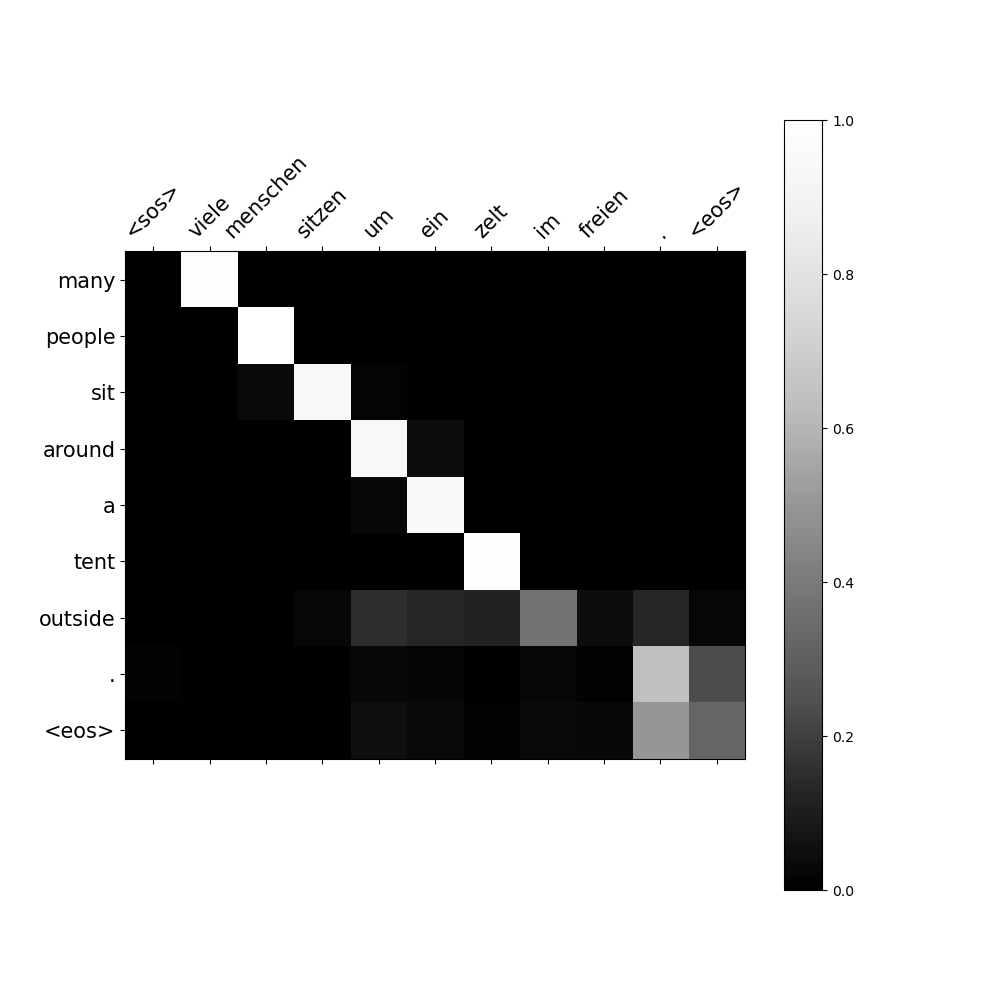
\includegraphics[width=0.5\textwidth]{figures/ex2.png}
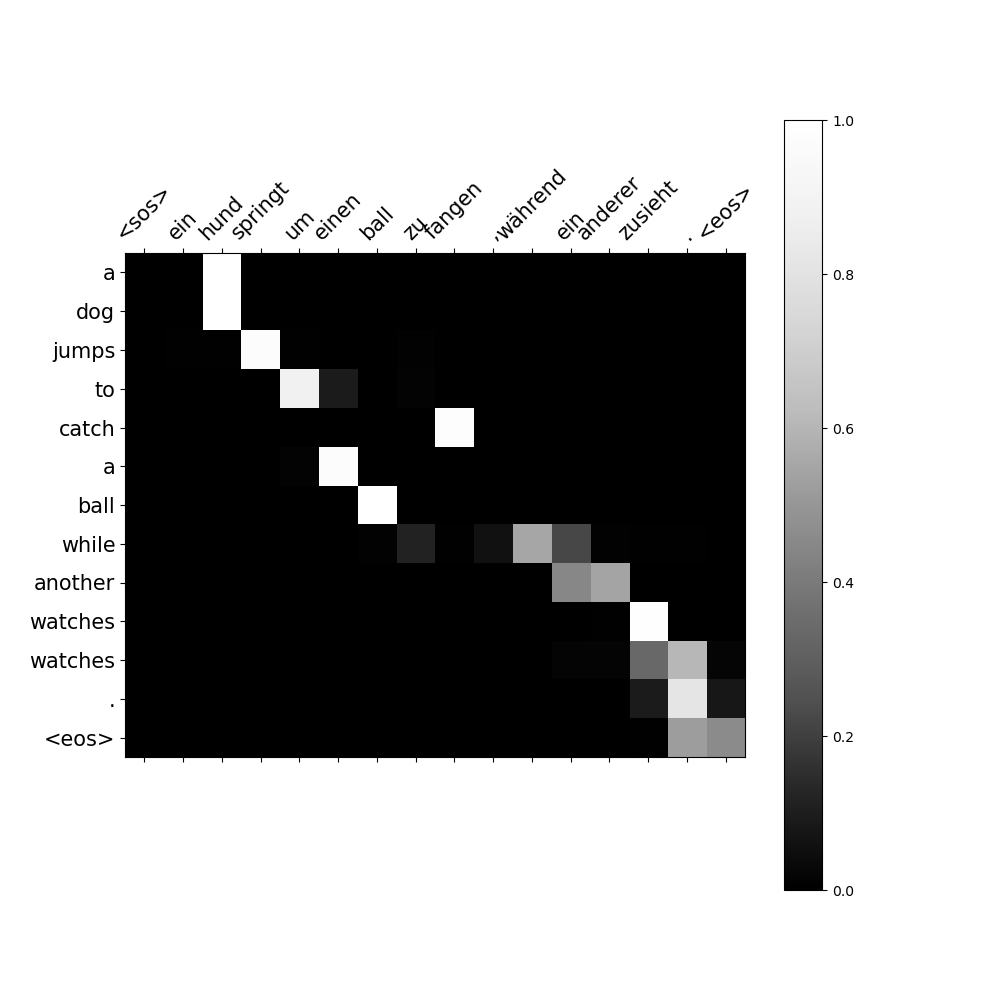
\includegraphics[width=0.5\textwidth]{figures/ex4.png}

\noindent where the brighter blocks indicate high attention values over source word encodings (columns) used when generating translated words (rows). Remember that these encodings also carry information about the rest of the sentence as they come from the bidirectional encoder.

\vspace{5pt}
\begin{taskbox}
\task{2.2 Attention Diagrams [1pts]}{ Search through the attention diagrams produced by your model. Include a few examples in your report and characterize common patterns you observe.Note that German is (mostly) a Subject-Object-Verb language so you may find attention patterns that indicate inversion of word order when translating to Subject-Verb-Object English as in the 2nd example above.}
\end{taskbox}
\vspace{5pt}

The code also implements two baseline options for the attention mechanism. A \texttt{Dummy} attention that just outputs zero tensors -- this effectively attends to \emph{no} words. The \texttt{MeanPool} attention which just averages the source word encodings -- this effectively attends \emph{equally} to all words. The code will use these if run with the \texttt{-{}-attn none} and \texttt{-{}-attn mean} arguments respectively.

\vspace{5pt}
\begin{taskbox}
\task{2.3 Comparison [3pts]}{ Train and evaluate models with the \texttt{Dummy} and \texttt{MeanPool} `attention' mechanisms. Report mean and variance over three runs for these baselines and your implementation of scaled dot-product attention. Discuss the observed trends.}
\end{taskbox}
\vspace{5pt}

\vspace{5pt}
\begin{taskbox}
\task{2.EC Beam Search and BLEU [2pts]}{This is an extra credit question and is optional.\\[8pt]

In the previous homework, we implemented many decoding algorithms; however, in this work we just use greedy top-1 in the \texttt{translate\_sentence} function. Adapt your implementation of beam search from HW3 to work on this model by augmenting \texttt{translate\_sentence} (which is used when computing BLEU).  Report BLEU scores on the test set for the scaled dot-product attention model with B=5, 10, 20, and 50.}
\end{taskbox}
\vspace{5pt}


%\section{Additional Resources}
%\vspace{20pt}
\renewcommand{\section}[2]{ {\hspace{-20pt}\color{blue!60}{\Large #2}} }

\bibliography{refs}
\bibliographystyle{ieeetr}
    
\end{document}
